\documentclass[../ECON-281-Notes.tex]{subfiles}
\begin{document}
\chapter{Input and Production Functions}
In this chapter we will look at 
\begin{itemize}
    \item Production in short run 
    \item Production in long run 
    \item Elasticity of substitution 
    \item Returns to scale
\end{itemize}

We will assume that we only have two inputs
\begin{itemize}
    \item Labour denoted as $L$
    \item Capital denoted as $K$
\end{itemize}
\begin{Definition}
    {Production Function}
    The production function for any supply or producer is so:
    \begin{equation}
        Q = f(L, K)
    \end{equation}
\end{Definition}

\section{Production in Short Run}
In the short run capital is fixed because it takes a long time to buy and sell expensive capital assets like land, machines, etc.
Only labour is variable because it's relatively easy to hire and fire workers in the short run. 

\begin{figure}[!ht]
    \centering
    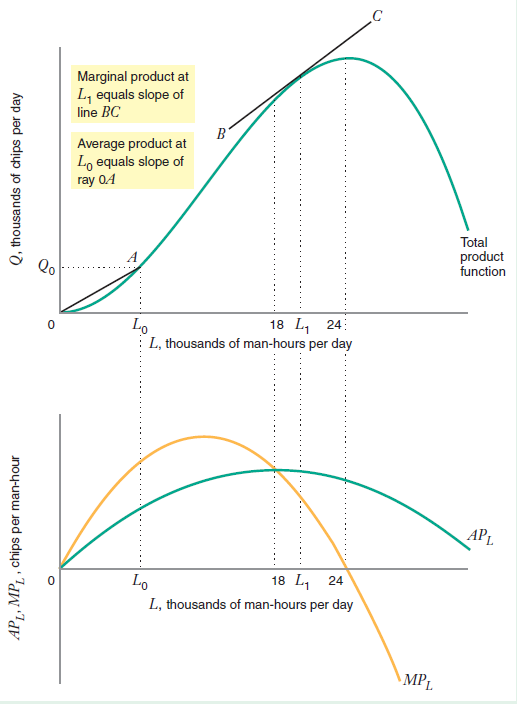
\includegraphics[width=\columnwidth]{../assets/Production_graphs.png}
    \caption{Product Graphs}
    \label{fig:product_graphs}
\end{figure}

In \cref{fig:product_graphs} we have two graphs one that shows total output for labour as input and another showing the \textbf{Marginal Production of Labour} and the \textbf{Average Production of Labour}. 
Both are calculated as so
\begin{equation}
    MP_L = \frac{\Delta Q}{\Delta L}    
\end{equation}
\(MP_L\) calculates the extra output from one extra unit of labour.
\begin{equation}
    AP_L = \frac{Q}{L}  
\end{equation}
\(AP_L\) calculates the average output per unit of labor.

\begin{Theorem}
    {Law of Diminishing Returns}
    Both \(MP_L\) and \(AP_L\) will eventually diminish as we have more units of labour beside a fixed amount of capital. 
\end{Theorem}

\section{Production in Long Run}
In the long run both \textbf{Labour} and \textbf{Capital} are variable and we have an equivalent indifference curve for production input. It's called \textbf{iso-quant}.

\begin{Definition}
    {Iso-quant}
    Shows different bundles of \(L\) and \(K\) that produce the same level of output.
    On the same iso-quant curve, the level of output is constant. The higher the iso quant curve the higher the level of output.

    Like indifference curves, iso-quant curves do not intersect and are convex to the origin. 
\end{Definition}
\begin{figure}[!h]
    \centering
    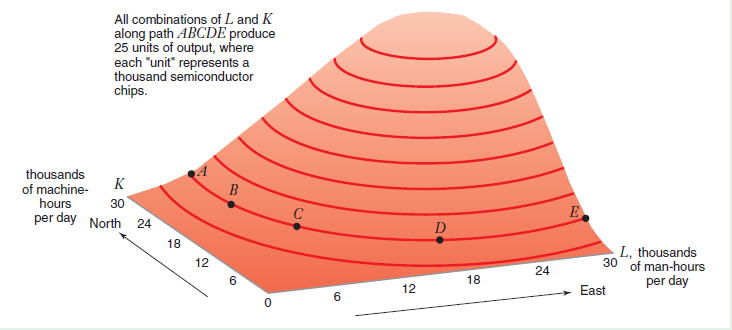
\includegraphics[width=\columnwidth]{../assets/isoquant.png}
    \caption{A map of Iso-quant}
    \label{fig:isoquant}
\end{figure}

\begin{Definition}
    {Marginal Rate of Technical Substitution MRTS}
    Is the slope of the iso-quant. It tells what we have to give up from one of the inputs to get an extra unit from the other input. Like MRS there are two versions. 

    \begin{equation}
        MRTS_{LK} = \frac{-\Delta K}{\Delta L} = \frac{-MP_L}{MP_K}
    \end{equation}
    \begin{equation}
        MRTS_{KL} = \frac{-\Delta L}{\Delta K} = \frac{-MP_K}{MP_L}
    \end{equation}
    
    Where:
    \begin{equation}
        MP_L = \frac{\partial Q}{\partial L}   
    \end{equation}
    \begin{equation}
        MP_K = \frac{\partial Q}{\partial K}
    \end{equation}
\end{Definition}

\begin{Theorem}
    {Law of Diminishing MRTS}
    We give up less and less from one input to get an extra unit from the other input. This means MRTS is diminishing. 
\end{Theorem}

\subsection{Difference cases of Iso-quants}
Like indifference curves there are 4 differeent cases
\begin{enumerate}
    \item Cobb-Douglas Production Function
    \item Perfect Complements (Leontief) Production Function
    \item Perfect Substitution (Linear) Production Function 
    \item Quasilinear Production Function 
\end{enumerate}
You can review that section of the notes and replace indifference curves with iso-quants and goods \(X\) and \(Y\) with \(L\) and \(K\).
\section{Elasticity of Substitution \(\sigma\) } 
It measures how easy for the firm to substitute labour for capital. 
The formula for which is so 
\begin{equation}
    \sigma = \frac{\% \Delta \frac{K}{L}}{\% \Delta MRTS_{LK}}
\end{equation} 
Where the range is between \(0\) and \(\infty\).
The higher the value of \(\sigma\), the easier it is to substitute one input for another. 

\subsection{Constant Elasticity of Substitution Production Function}
Each of the three production functions we have discussed is a special case of a production function called the \textbf{constant elasticity of substitution} (CES) production function, which is given by the equation:
\begin{equation}
    Q = [aL^{\frac{\sigma - 1}{\sigma}} + bK^{\frac{\sigma - 1}{\sigma}} ]^{\frac{\sigma}{\sigma - 1}} 
\end{equation}
Where \(a\) and \(b\) are positive constant numbers and \(\sigma\) is the elasticity of substitution that is constant.

\begin{figure}[h]
    \centering
    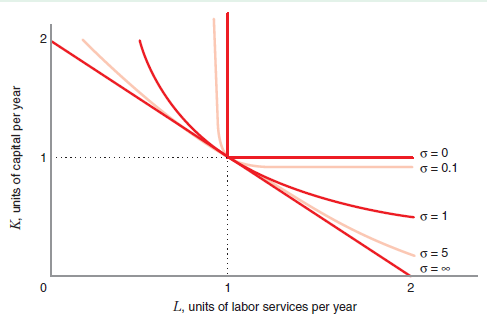
\includegraphics[width=\columnwidth]{../assets/CES_isoquants.png}
    \caption{Elasticity of Substitution}
    \label{fig:elasticity_sub}
\end{figure}

\begin{DndTable}[color=PhbLightGreen]{XX}
    \textbf{Production Function} & \textbf{Elasticity of Substitution} \\
    Linear Production Function & \(\sigma = \infty\) \\
    Perfect Complement Production Function & \(\sigma = 0\) \\
    Cobb-Douglas Production Function & \(\sigma = 1\)
\end{DndTable}

\section{Return to Scale}
\begin{Definition}
    {Return to Scale}
    RTS measures what happens to output \(Q\) when all inputs changes by the same \%.
\end{Definition}

\begin{figure}[h]
    \centering
    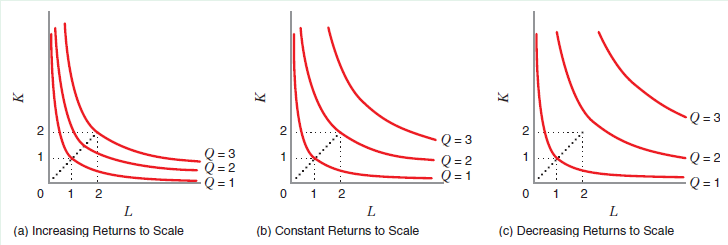
\includegraphics[width=\columnwidth]{../assets/RTS.png}
    \caption{Return to Scale}
    \label{fig:RTS}
\end{figure}

\begin{itemize}
    \item \(\% \Delta Q > \% \Delta inputs\) - Increasing RTS 
    \item \(\% \Delta Q = \% \Delta inputs\) - Constant RTS 
    \item \(\% \Delta Q < \% \Delta inputs\) - Decreasing RTS 
\end{itemize}


\end{document}